\subsection{Image Meter}

\subsubsection{Vorstellung}
Die App \im{} von \emph{Dirk Farin} hat zur Zeit des Downloads (20. Januar 2018) bei insgesamt 2 764 abgegeben Bewertungen eine durchschnittliche Bewertung von 3,9 von 5 Sternen im Google Play-Store \citep{FarinIM}.
Hierbei haben 72\% (1978) der Bewertungen vier oder fünf, und nur 28\% (786) 3 oder weniger Sterne.
Dies ist eine überdurchschnittlich hohe Bewertung, und macht die App zu einer der Beliebtesten unter dem Suchbegriff ``Aufmaße''.
Der Entwickler selbst beschreibt die App im Play-Store wie folgt \citep{FarinIM}:

\begin{quote}
  ``ImageMeter erlaubt das Beschriften Ihrer Fotos mit Längen-, Winkel- und Flächenmaßen sowie Text.
  Das ist viel einfacher und anschaulicher als aufwändig eine Skizze zu zeichnen.''
\end{quote}

\noindent
\begin{wrapfigure}{R}{0.5\textwidth}
  \centering
  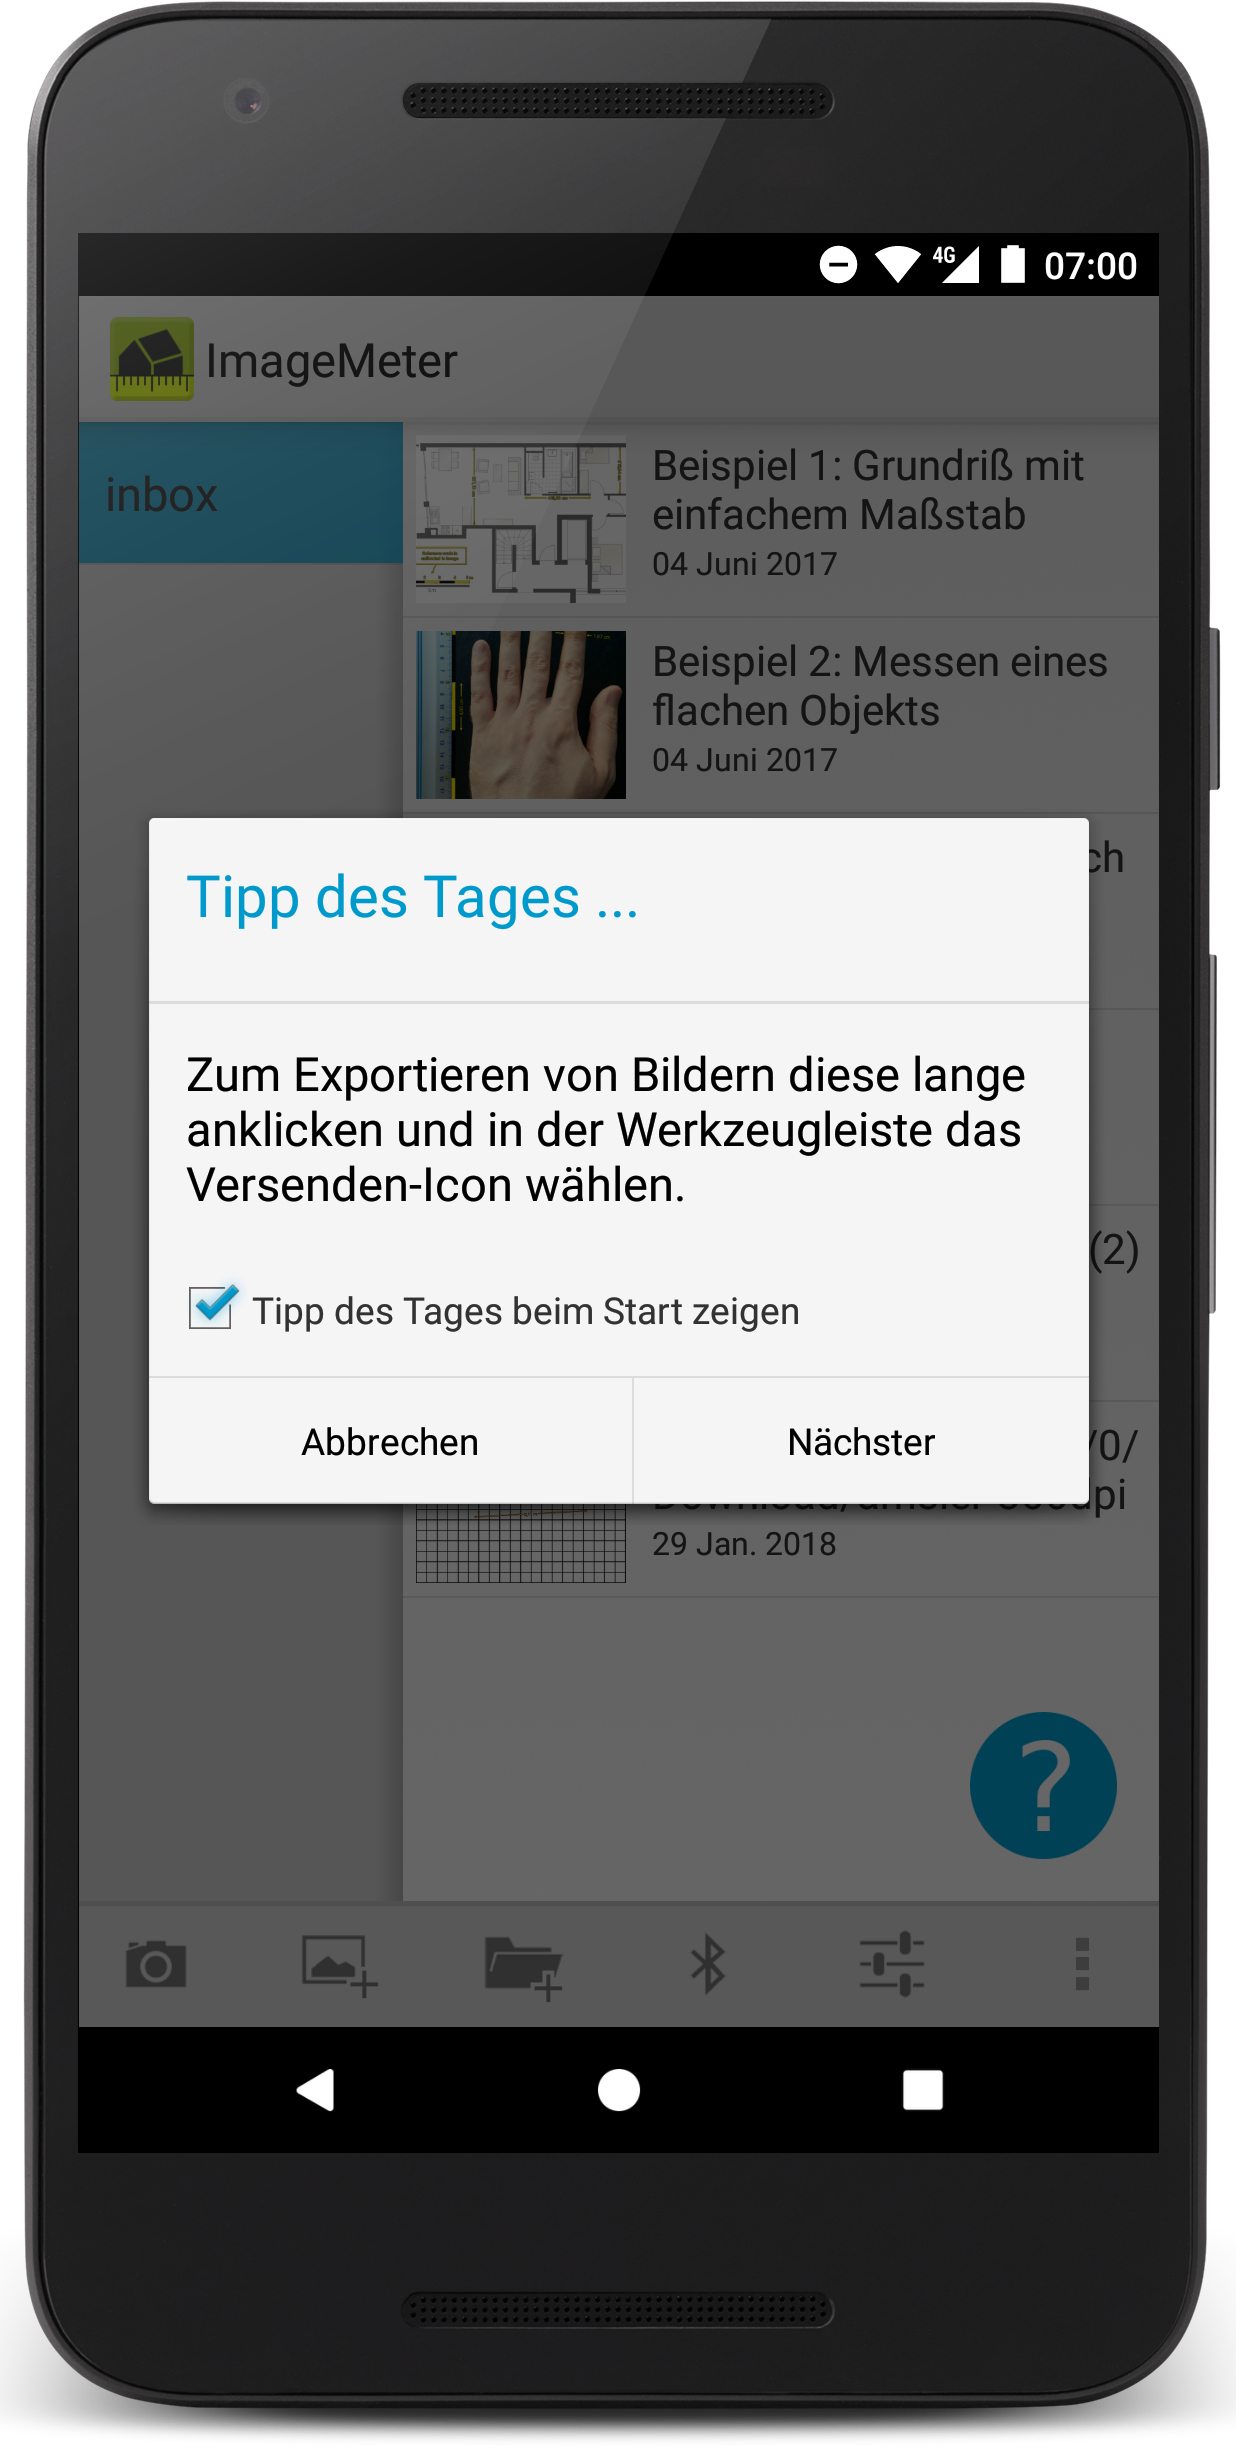
\includegraphics[keepaspectratio, width=0.5\textwidth]{image_meter/tip}
  \caption{``Tipp des Tages'' beim Start der App}
  \label{fig:imtip}
\end{wrapfigure}
Beim Start der App wird dem Benutzer der sogenannte ``Tipp des Tages'' angezeigt.
Dieser enthält Informationen zu bestimmten Funktionen der App, wie zum Beispiel dem Exportieren von Bildern (siehe \autoref{fig:imtip}).
Hier hat der Nutzer die Möglichkeit sich weitere Tipps anzusehen, oder diese durch das Entfernen des Hakens in der Checkbox ``Tipp des Tages beim Start zeigen'' dauerhaft zu deaktivieren. \\

Sobald der Dialog zum ``Tipp des Tages'' geschlossen wurde, bietet sich über die Statusleiste am unteren Bildschirmrand die Möglichkeit, ein neues Bild aufzunehmen, oder direkt eines aus der Galerie zu importieren (siehe \autoref{fig:immenu}). \\

Das ausgewählte Bild wird nach erfolgreichem Import in die App im Hauptmenü in einer Liste mit alleren weiteren Bildern angezeigt.
Hier gelangt der Benutzer durch einen Klick auf das gewünschte Bild in eine neue Bildschirmoberfläche, in der das Bild beschriftet werden kann (siehe \autoref{fig:imdraw}).
In dieser Oberfläche wird dem Nutzer das zuvor ausgewählte Bild und eine neue Statusleiste am unteren Bildschirm angezeigt.
Oberhalb der Statusleiste befindet sich ein ``Floating Action Button'' (\emph{FAB}), der durch ein Fragezeichen-Icon gekennzeichnet ist.
Der \emph{FAB} öffnet beim Klick auf sich eine separate Hilfe-Seite, in der häufig gestellte Fragen und deren Antworten zu den Funktionen der App beschrieben stehen. \\

Zusätzlich zu dieser Hilfestellung, wird dem Benutzer beim Auswählen des Zeichen-Modus ein erklärender Text über der Statusleiste angezeigt (siehe \autoref{fig:imdraw}).
Dieser beschreibt genau, welche Aktion der Nutzer im aktuellen Systemzustand durchführen kann bzw. soll. \\

\begin{figure}[h]
  \centering
  \begin{subfigure}[t]{0.4\textwidth}
    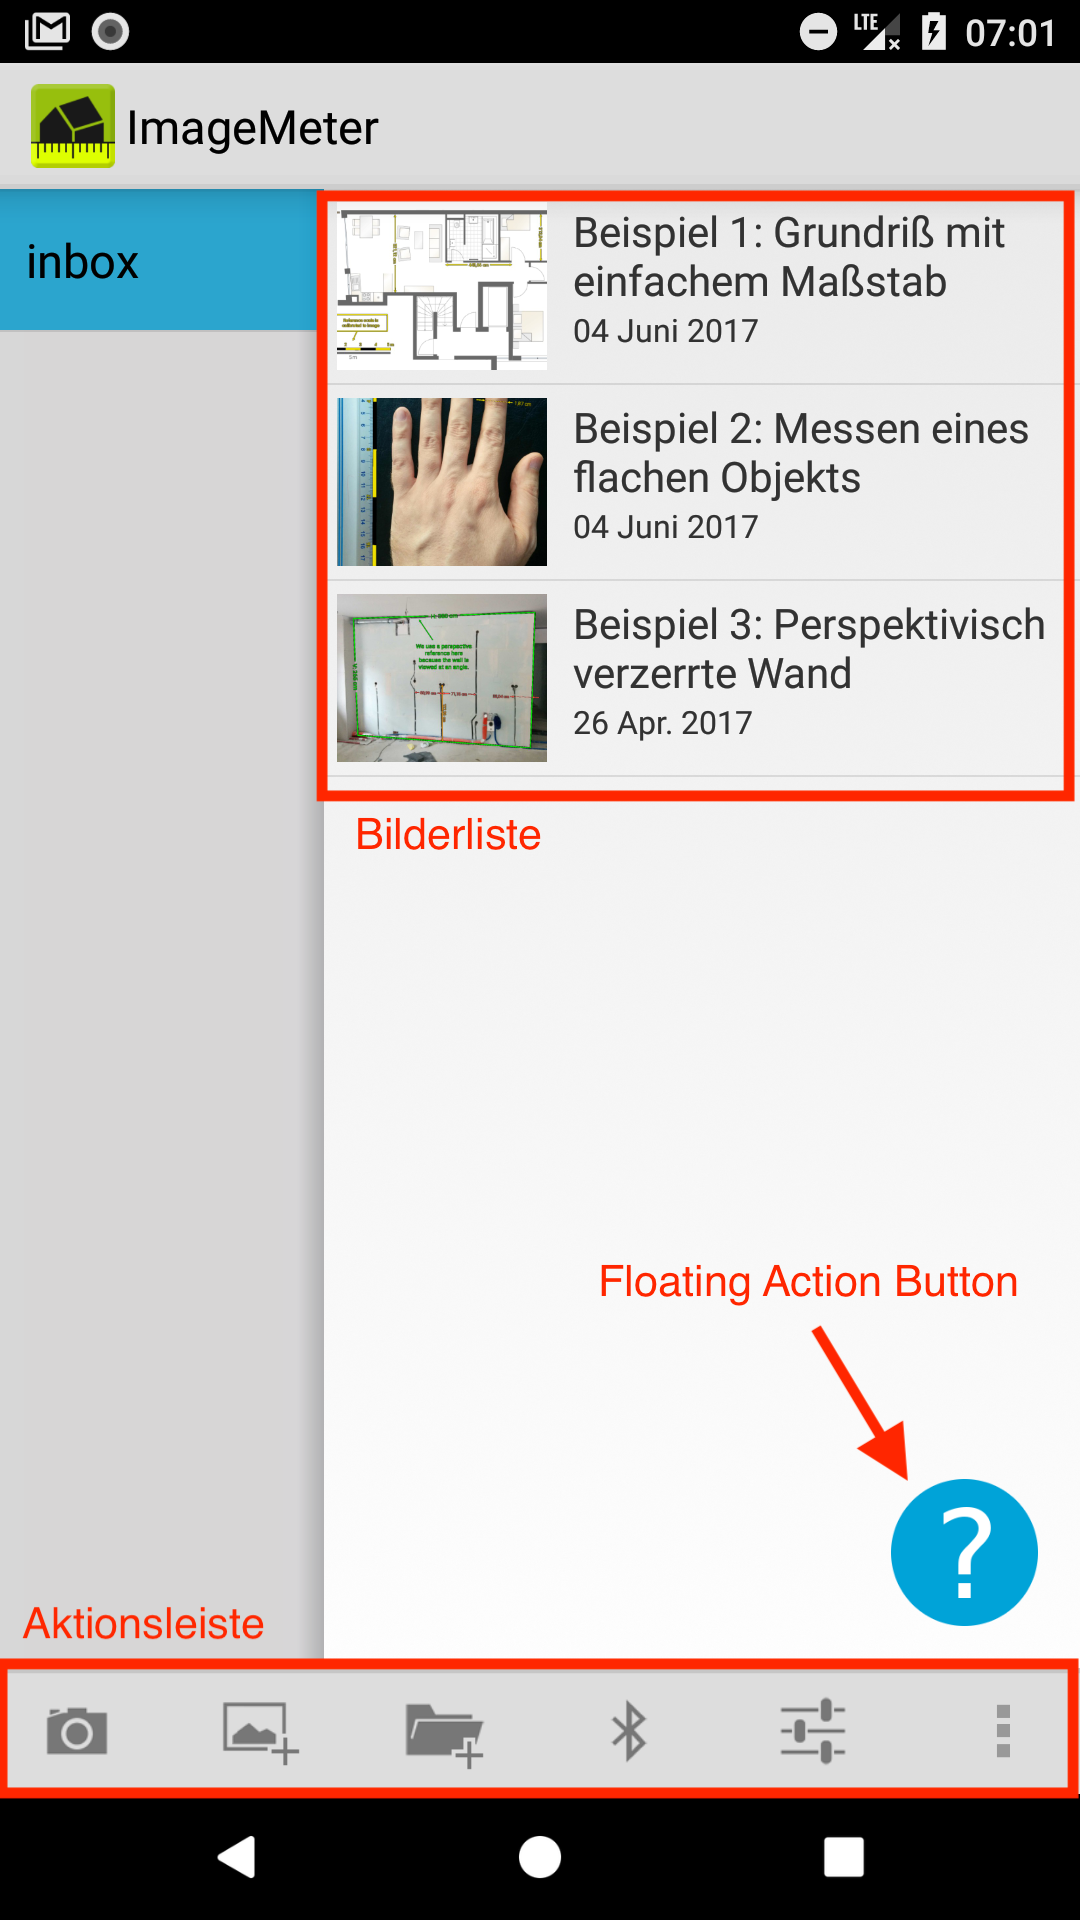
\includegraphics[keepaspectratio, width=\textwidth]{image_meter/menu}
    \caption{Hauptansicht der App}
    \label{fig:immenu}	
  \end{subfigure}
  \begin{subfigure}[t]{0.4\textwidth}
    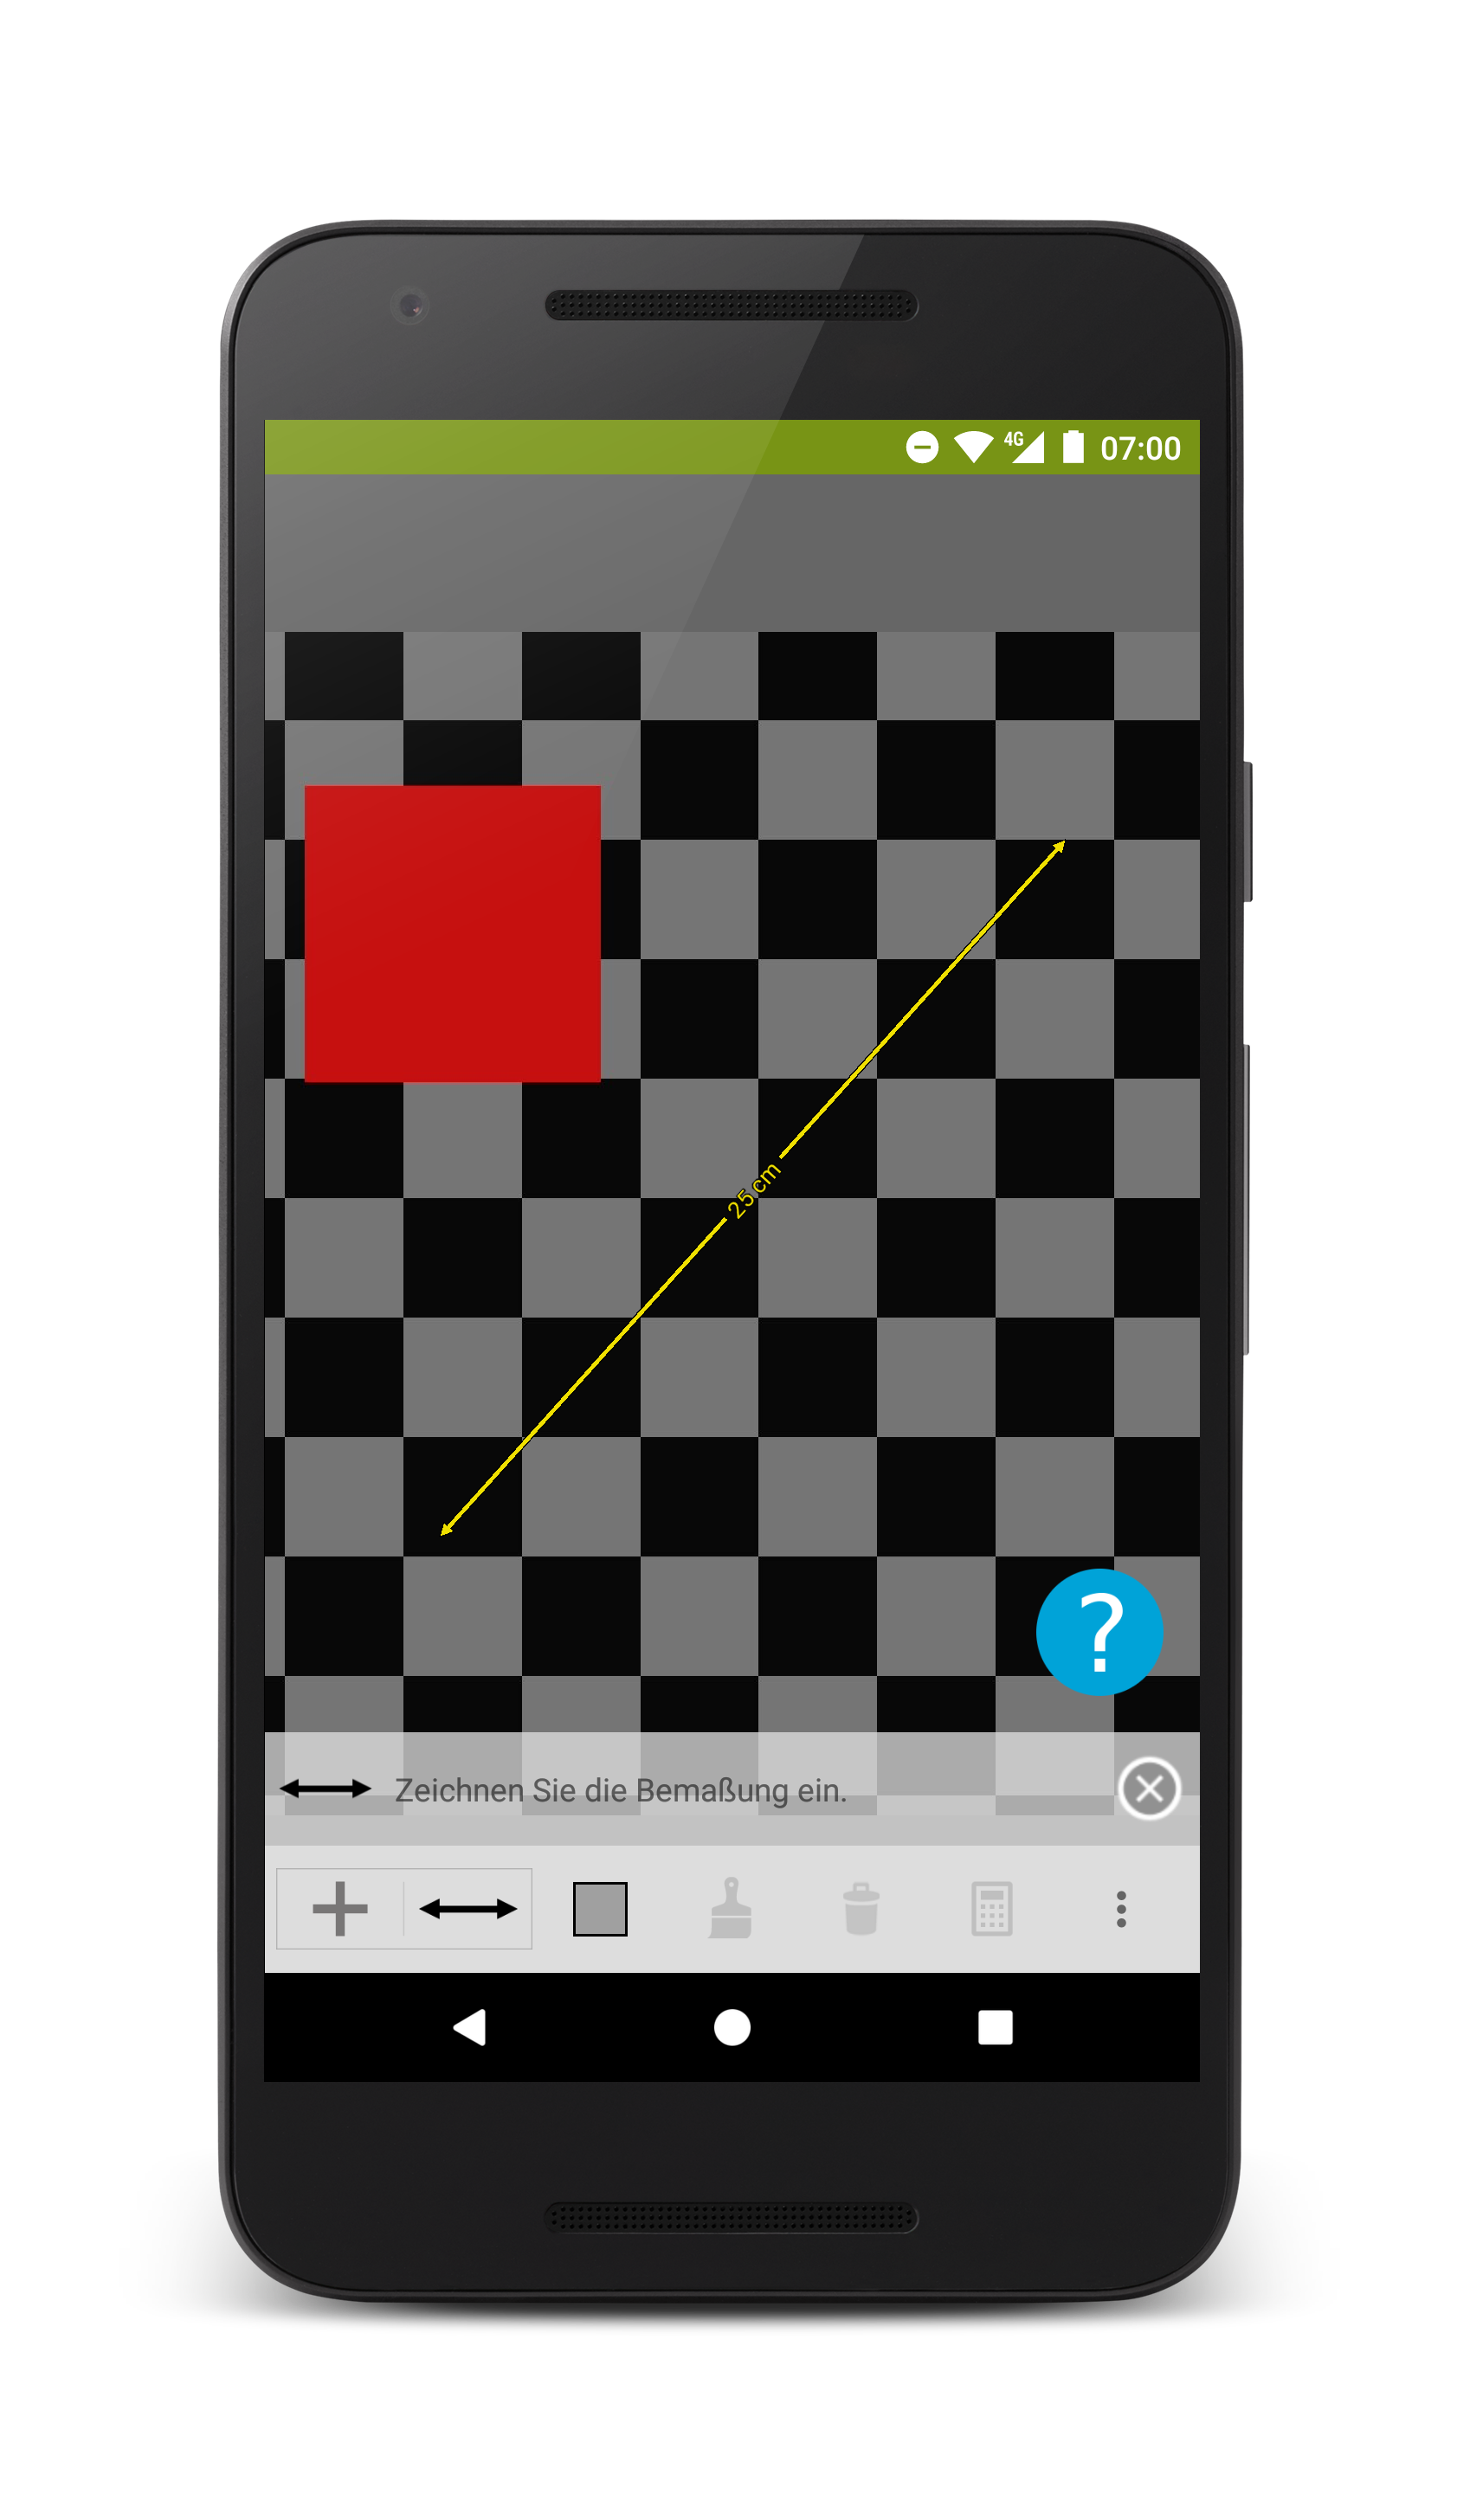
\includegraphics[keepaspectratio, width=\textwidth]{image_meter/draw}
    \caption{Aufmaße-Funktion mit eingezeichneter Form} 
    \label{fig:imdraw}	
  \end{subfigure}
  \caption{\im{} nach dem Start der App und in der Aufmaß-Funktion}
\end{figure}

\noindent
Die Statusleiste bietet dem Nutzer außerdem die Möglichkeit, die gewünschte Form und deren Farbe festzulegen.
Die Farbe bereits eingezeichneter Formen kann auch noch im Nachhinein angepasst werden.
Zu jeder Zeit sind nur die Funktionen in der Statusleiste auswählbar, die im aktuellen Systemzustand durchführbar sind.
So ist bspw. das Löschen von Formen nur dann möglich, wenn zuvor eine Form markiert wurde. \\

Insgesamt kann der Nutzer aus bis zu sieben verschiedene Formen (zehn in der Pro-Version) frei auswählen.
Unter diesen sieben Formen der Free-Version befinden sich auch zwei Referenz-Formen.
Diese können dazu genutzt werden, um Referenzlängen im Bild festzulegen, und ermöglichen so, dass alle nachträglich eingezeichneten Formen automatisch mit Messwerten versehen werden. \\

Eine Undo- bzw. Redo-Funktion ist über das \emph{Overflow-Menü} in der Statusleiste erreichbar.
Hierdurch können ausgeführte Aktionen rückgängig gemacht oder wiederholt werden. \\

Auch in dieser App lassen sich gespeicherte Bilder zu einem späteren Zeitpunkt weiter bearbeiten.
Außerdem können mehrere Bilder gleichzeitig zusammen in einer \emph{PDF} exportiert werden.

\subsubsection{Evaluation}\label{subsec:imeva}
Hilfe und Dokumentation (Nielsen~\autoref{itm:N10}) werden in dieser App in Form des ``Tipp des Tages'' (siehe \autoref{fig:imtip}) und die dedizierte Hilfe-Oberfläche bereit gestellt.

\begin{wrapfigure}{R}{0.5\textwidth}
  \centering
  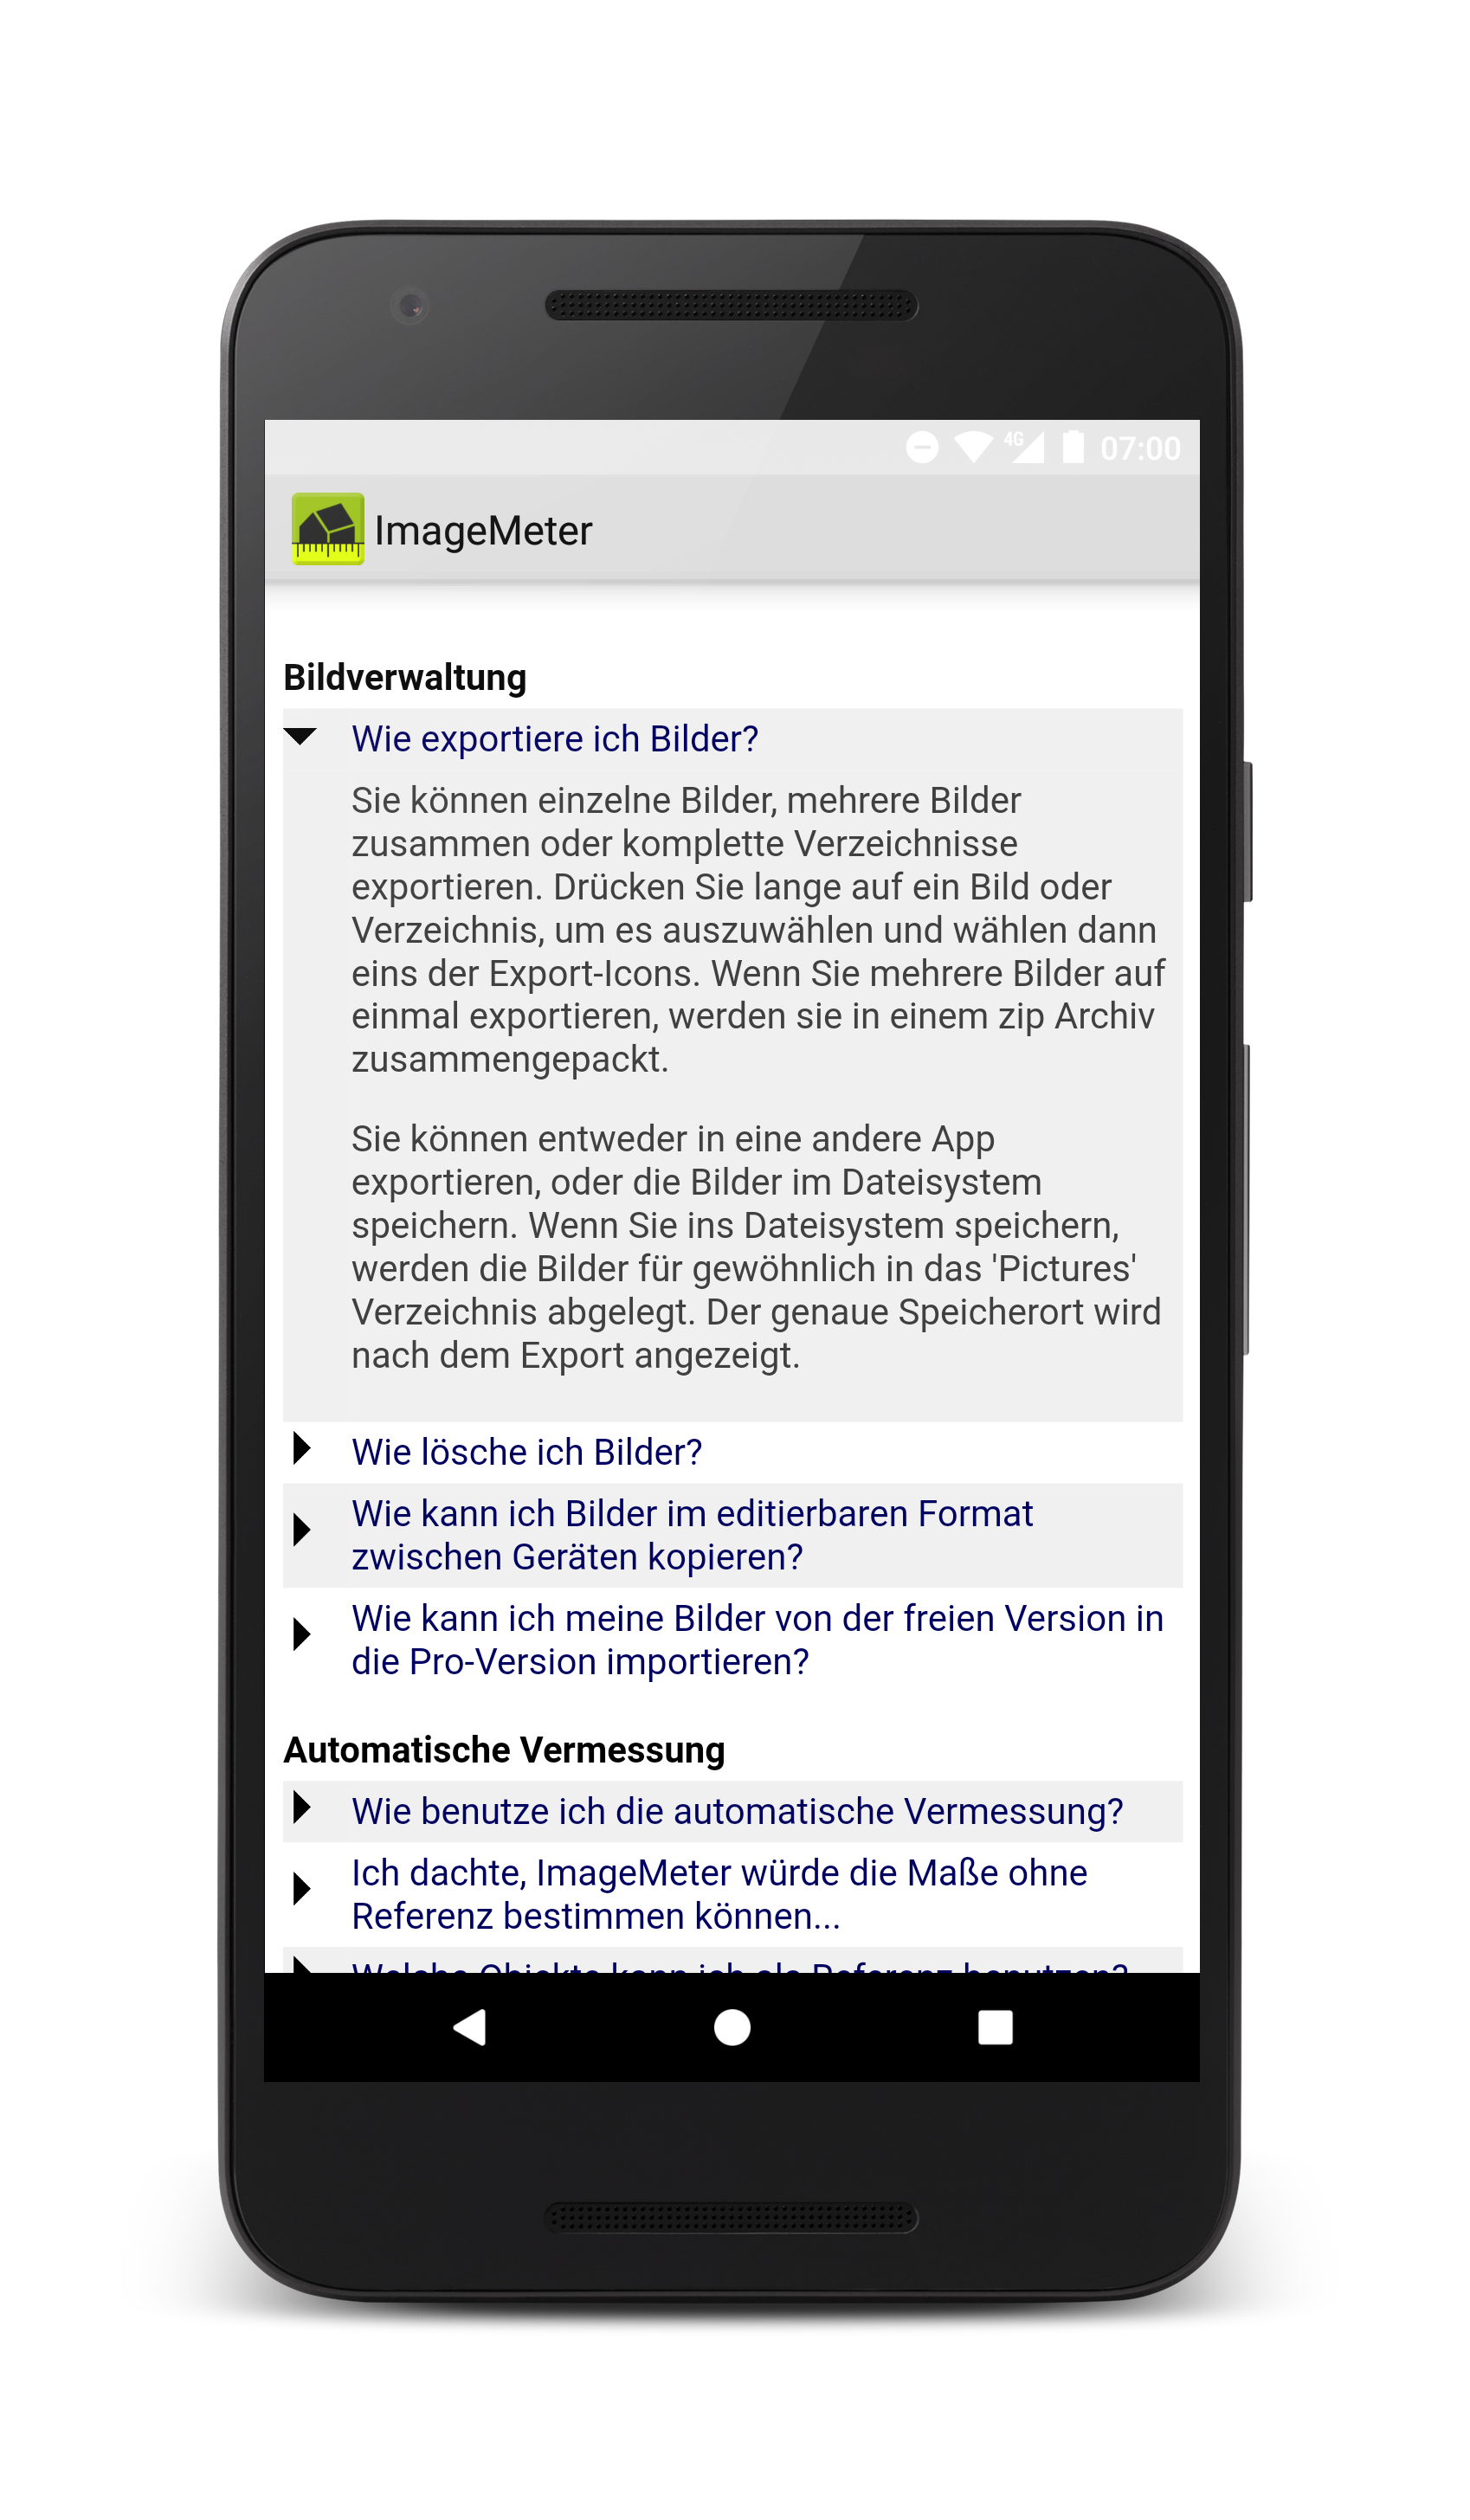
\includegraphics[keepaspectratio, width=0.5\textwidth]{image_meter/faq}
  \caption{Hilfeoberfläche der App}
  \label{fig:imfaq}
\end{wrapfigure}

Hierbei bietet die Hilfe-Oberfläche eine Liste von Fragen und Antworten zu den verschiedenen Funktionen der App an (siehe \autoref{fig:imfaq}). \\

Die Statusleiste zeigt zu jedem Zeitpunkt den ausgewählten Modus und die darin ausführbaren Aktionen an.
Hierdurch gibt die App dem Nutzer eine angemessene und verständliche Rückmeldung über den aktuellen Systemzustand der App (Nielsen~\autoref{itm:N1} \& \autoref{itm:N5}). \\

Formen können, nachdem sie in das Bild gezeichnet wurden, zu einem späteren Zeitpunkt in ihrer Farbe und Größe verändert werden.
Zusätzlich dazu gibt es in den Einstellungen der App weitere Möglichkeiten, die App an die eigenen Bedürfnisse anzupassen.
So kann unter anderem eingestellt werden, ob Maßeinheiten angezeigt werden sollen, welche metrischen Einheiten benutzt werden sollen, oder wie viele Dezimalstellen für Messwerte verwendet werden solle.
Dies erlaubt nicht nur eine flexible Benutzung der App, sondern kann gleichzeitig zu einer effizienteren Nutzung führen, da die App nur einmal zu Beginn konfiguriert werden muss (Nielsten~\autoref{itm:N7}) \\

Situationen, in denen Fehler entstehen könnten, werden von der App präventiv vermieden.
Hierzu werden Aktionen, die beim Ausführen im aktuellen Systemzustand zu einem Fehler führen würden, ausgegraut und sind in der Statusleiste nicht auswählbar (Nielsen~\autoref{itm:N5} \& \autoref{itm:N9}). \\

\begin{wrapfigure}{R}{0.5\textwidth}
  \centering
  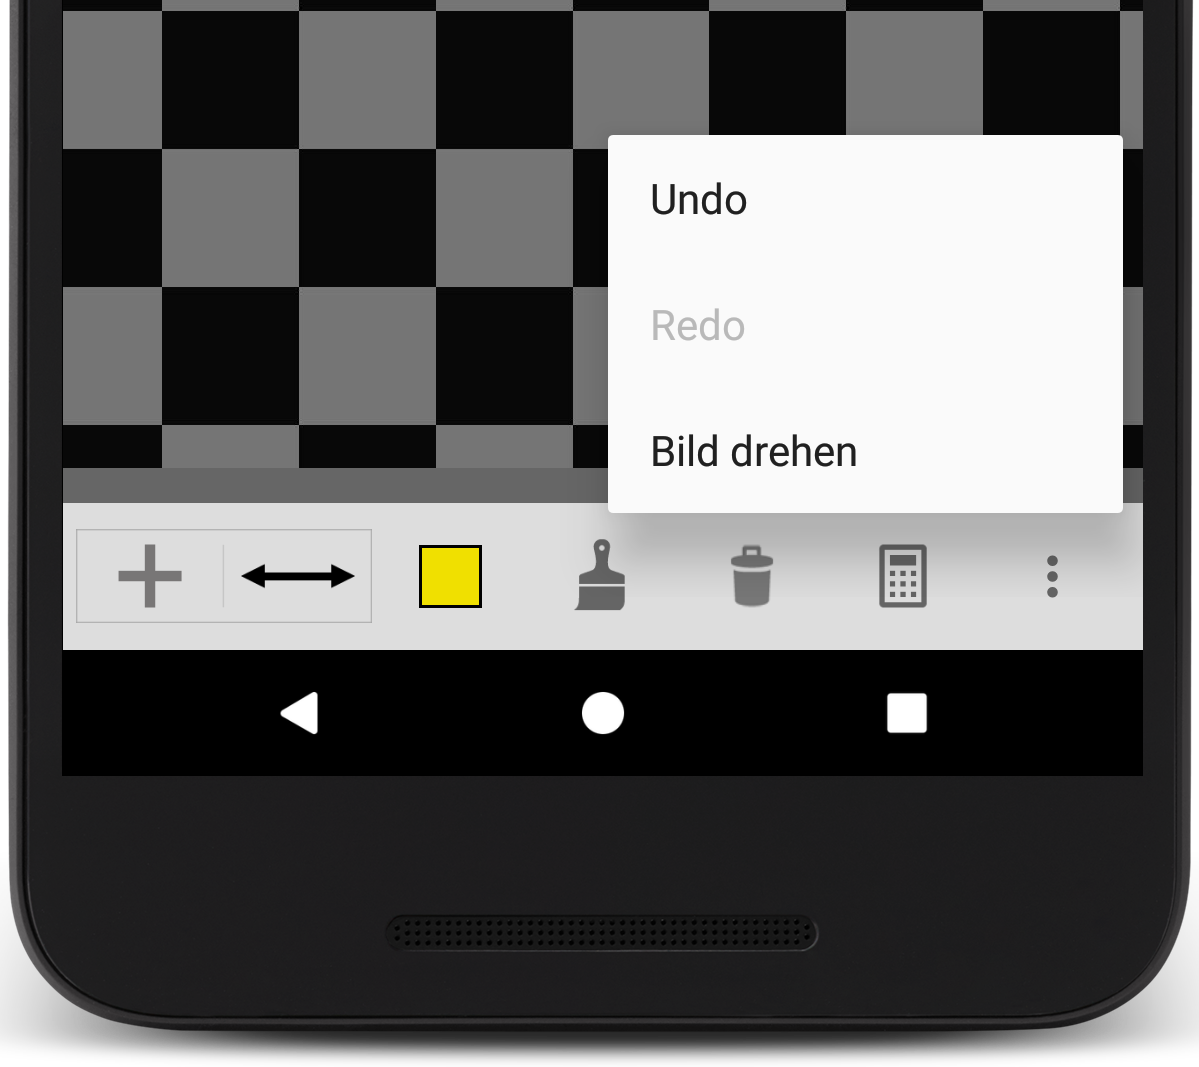
\includegraphics[keepaspectratio, width=0.5\textwidth]{image_meter/bar}
  \caption{Statusleiste in der Aufmaßfunktion}
  \label{fig:imbar}
\end{wrapfigure}

Das Ausgrauen der deaktivierten Icons kann jedoch in Kombination mit den anderen verwendeten Farben in der Statusleiste zu Verwirrung führen.
So werden hier nicht nur deaktivierte Icons grau eingefärbt, sondern auch die anderen Icons in einem ähnlichen Grauton dargestellt (siehe \autoref{fig:imbar}).
Hier wird nicht deutlich, ob das Plus-Icon (ganz links) zur Zeit deaktiviert oder aktiviert ist, weil es in einem ähnlichen Grauton wie die deaktivierten Icons auf der rechten Seite dargestellt wird.
Diese Verwirrung wird zusätzlich durch die Icon-Farbe der ausgewählten Form (zweites Icon von links) verstärkt.
Für dieses Icon wird nämlich eine schwarze Farbe verwendet. \\

Fehlerhafte oder ungewollte Eingaben kann der Nutzer über den Undo- bzw. Redo-Button in der Statusleiste verbessern bzw. wiederholen (Nielsen \autoref{itm:N3}).
Bei der Benutzung der App im Hochformat sind diese beiden Buttons jedoch nicht direkt sichtbar, da sie in einem \emph{Overflow-Menü} an der rechten Seite der Statusleiste versteckt sind (siehe \autoref{fig:imbar}).
Der Benutzer muss hier also im Voraus wissen, dass sich dort die Optionen zum Undo bzw. Redo befinden. \todo{Schreiben, warum das ungünstig ist} \\

Ein positiver Aspekt dagegen liegt beim adäquaten Umgang mit Unterbrechungen, sowie der Unterstützung verschiedener Bildschirmausrichtungen (Nielsen~\autoref{itm:N11} \& \autoref{itm:N15}).
Beim Pausieren und Drehen der App werden alle bereits eingezeichnete Formen oder eingetragene Messwerte gespeichert, und das Bild bleibt stets in der erwarteten Ausrichtung.
Zudem wird die zusätzliche Bildschirmbreite, die sich bei der Benutzung im Querformat ergibt, dazu genutzt, um alle Elemente der Statusleiste anzuzeigen, ohne Aktionen in einem Overflow-Menü zu gruppieren. \todo{Bild von Statusleiste im Querformat} \\

\begin{wrapfigure}{R}{0.5\textwidth}
  \centering
  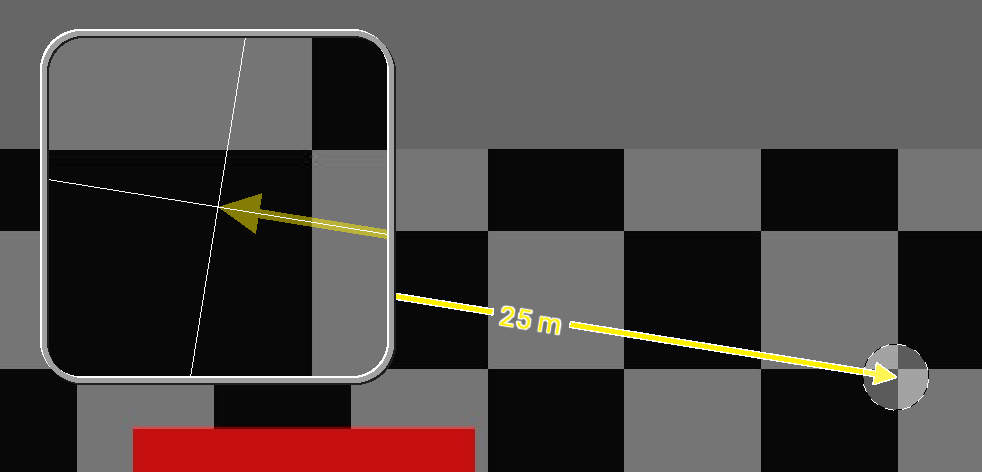
\includegraphics[keepaspectratio, width=0.5\textwidth]{image_meter/lensebug}
  \caption{Zoom-Linse verdeckt Zeichenbereich}
  \label{fig:imlense}
\end{wrapfigure}

Die Gesten-Unterstützung zur Navigation im Bild ist in dieser App problemlos möglich (Nielsen~\autoref{itm:N13}, \autoref{itm:N16} \& \autoref{itm:N17}).
Hier kann der Benutzer mit Hilfe einer \emph{Pinch-} oder \emph{Doppelklick-Geste} in das Bild herein- bzw. herauszuzoomen.
Um den Sichtbereich im Bild zu verschieben, kann eine \emph{Pan-Geste} genutzt werden.
Diese gute Umsetzung der Gesten-Unterstützung in Kombination mit einer effizienten einhändigen Handhabung der App führen zu einem deutlich positiven Anwendererlebnis. \todo{Irgendwo vorher die verschiedenen Gesten erklären} \\

Auch diese App bedient sich beim Zeichnen von Formen einer Zoom-Linse, welche den Bereich um die Fingerposition vergrößert darstellt.
Negativ fällt bei der Umsetzung dieser Funktion jedoch auf, dass die Zoom-Linse statisch in der oberen linken Ecke angezeigt wird, und sich bei einer Kollision mit dem Finger nicht bewegt.
So kann es passieren, dass die Zoom-Linse beim Zeichnen einer Form den gewünschten Zeichenbereich verdeckt, und der Benutzer nicht sieht, wo genau die Form eingezeichnet wird.
Die Zoom-Linse verfehlt also in dieser Umsetzung ihre eigentlichen Aufgabe als Hilfestellung zum genaueren und schnelleren Zeichnen der Formen (siehe \autoref{fig:imlense}). \\

Der Export von eingetragenen Messwerten als Meta-Daten ist auch in dieser App nicht möglich.
So bietet die App zwar die Möglichkeit Bilder aus einer bestehenden App an diese zu teilen, stellt beim anschließenden Exportieren der bearbeiteten Bilder jedoch keinerlei Meta-Daten zur Weiterverarbeitung in einem nachgelagerten Dienst wie einer \emph{API} bereit (\autoref{itm:export}). \\

Zusammenfassend kann festgehalten werden, dass die App \im{} von \emph{Dirk Farin} die Nielsen-Heuristiken überwiegend positiv erfüllt.
Besonders die gute Umsetzung der Gesten-Unterstützung sorgt für ein positives Nutzungserlebnis.
Negativ fallen jedoch die versteckte Undo- und Redo-Funktion im \emph{Overflow-Menü} und die Verwirrung des Nutzers durch die Verwendung ähnlicher Grautöne für unterschiedliche Aktionen in der Statusleiste auf.
Zudem fehlt eine initiale Hilfestellung beim Wechsel in die Aufmaß-Oberfläche.
Hier muss der Benutzer zuerst in eine andere Benutzeroberfläche wechseln und die passende Antwort suchen, falls sich Fragen während des Zeichnens von Formen ergeben.
Die Integration in eine bestehende Systemarchitektur ist auch bei dieser App nicht ohne Weiteres umsetzbar, da alle eingetragenen Messwerte beim Exportieren der Bilder nicht mehr als Meta-Daten vorhanden sind.
\todo{Schreiben, dass Tipp des Tages schlecht umgesetzt, weil nur 3 statische Tipps (Wiederholung)}
